\documentclass[%
 %reprint,                 % retiré : l'en-tête d'origine n'utilisait pas reprint
 superscriptaddress,
 amsmath,amssymb,
 aps,
 pra,                      % pre -> pra (comme l'en-tête d'origine)
 floatfix,
]{revtex4-2}

% --- Encoding and language ---
\usepackage[utf8]{inputenc}
\usepackage[T1]{fontenc}
\usepackage[english]{babel}
\usepackage{microtype}
\usepackage{xspace}
\usepackage{xcolor}

% --- Mathematics and symbols ---
\usepackage{mathrsfs, stmaryrd}
\usepackage{amsfonts}
\usepackage{siunitx}
\usepackage{bm}
\DeclareMathOperator\arctanh{arctanh}

% --- Graphics and figures ---
\usepackage{graphicx}
\usepackage{float}        % option [H]
\usepackage{caption}
\usepackage{subcaption}   % si problème avec revtex, utiliser \usepackage{subfig}
\graphicspath{{pictures/}}
\usepackage{placeins}     % pour \FloatBarrier

\captionsetup[figure]{justification=raggedright, singlelinecheck=false, format=plain}
\captionsetup[subfigure]{justification=centering}

% --- Float placement ---
\setcounter{topnumber}{3}
\setcounter{bottomnumber}{3}
\setcounter{totalnumber}{6}
\renewcommand{\topfraction}{0.9}
\renewcommand{\bottomfraction}{0.9}
\renewcommand{\textfraction}{0.1}
\renewcommand{\floatpagefraction}{0.7}
\setlength{\parskip}{0.5\baselineskip}

% --- Tables ---
\usepackage{booktabs}
\usepackage{multirow, array, makecell}
\usepackage{dcolumn}

% --- Lists ---
\usepackage{enumitem}

% --- Algorithms and code ---
\usepackage[ruled,vlined]{algorithm2e}
\usepackage{listings}
\usepackage{fvextra}
\usepackage{tikz}
\usetikzlibrary{decorations.pathreplacing}

% --- Text editing / review ---
\usepackage[normalem]{ulem}
\usepackage{lineno}

% --- References (hyperref avant cleveref) ---
\usepackage{hyperref}
\usepackage{cleveref}
\crefname{algocf}{algorithm}{algorithms}
\Crefname{algocf}{Algorithm}{Algorithms}
\bibliographystyle{apsrev4-2}

% --- Macros : annotations (à retirer avant soumission) ---
\newcommand{\note}[1]{\textcolor{blue}{#1}}
\newcommand{\noteBastien}[1]{\textcolor{blue}{#1}}
\newcommand{\noteMichele}[1]{\textcolor{red}{#1}}
\newcommand{\noteDavid}[1]{\textcolor{green}{#1}}

% --- Macros : code identifiers ---
\newcommand{\UnsignedInt}{\texttt{UnsignedInt}\xspace}
\newcommand{\UnsignedInts}{\texttt{UnsignedInts}\xspace}
\newcommand{\BitSet}{\texttt{BitSet}\xspace}
\newcommand{\BitSets}{\texttt{BitSets}\xspace}
\newcommand{\Bits}{\texttt{Bits}\xspace}

\begin{document}

We show in \Cref{fig:phase_transition} the evolution of the error with the storage load:
\nolinenumbers
\begin{figure}[h]
\centering
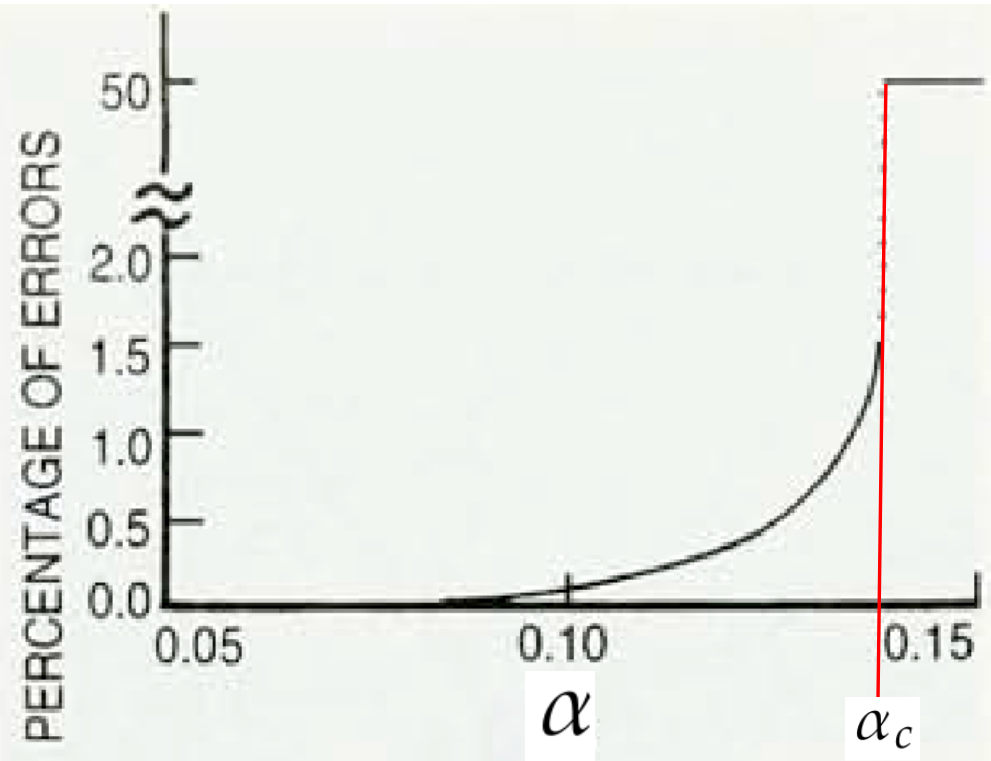
\includegraphics[width=0.6\columnwidth]{phase_transition.png}
\caption{Evolution of the error with the storage load, extracted from \cite{Sompolinsky1988}.  For this diagram, the configuration is initialized near a pattern. When the storage load exceeds $\alpha_c$, the configuration becomes totally uncorrelated with the stored patterns and the error suddenly jumps to 0.5.}
\label{fig:phase_transition}
\end{figure}
\linenumbers
The convention used for what follows is presented in the Table \ref{tab:notation}:
\nolinenumbers
\begin{table}[b]
\centering
\begin{tabular}{ll}
\hline
Object & Notation \\
\hline

$n_\text{bits}$ replicas of spin i & $S_i \in \{-1,1\}^{n_\text{bits}}$ \\
$n_\text{bits}$-bit word (\Bits) & $B_i \in \{0,1\}^{n_\text{bits}}$ \\
Replica $k$ of spin $i$ & $s_i^{(k)} \in \{-1,+1\}$ \\
Replica $k$ of bit $i$ & $b_i^{(k)} \in \{0,1\}$ \\
\hline
\end{tabular}
\caption{Notation for the bitwise representation of spins.}
\label{tab:notation}
\end{table}
\linenumbers
\end{document}
